Para analizar los algortimos implementados vamos a utilizar los archivos test1.in y test2.in provistos por la cátedra y realizar una serie de test que nos permitirán en primer caso encontrar parametros buenos con lo que ejecutarlos y posteriormente evaluar el desempeño de la implementación mediante las métricas propuestas por la cátedra.

Dividimos la experimentación en dos secciones, una para cada archivo de prueba. Y evaluaremos los parametros individualmente para cada una de ellas

\subsection {Algoritmo de K-NN}

Lo primero que vamos a hacer es encontrar un valor de $K$ que nos permita maximizar la cantidad de aciertos, sin tener en consideración las métricas.

Ejecutamos el algoritmos de $K-NN$ variando los valores de k entre {1..20} dejando fija la cantidad de particiones en 10. Luego para cada K nos quedamos con los resultados de la iteración con mas aciertos.

Expresamos los aciertos para cada K en con el siguiente gráfico:
\begin{center}
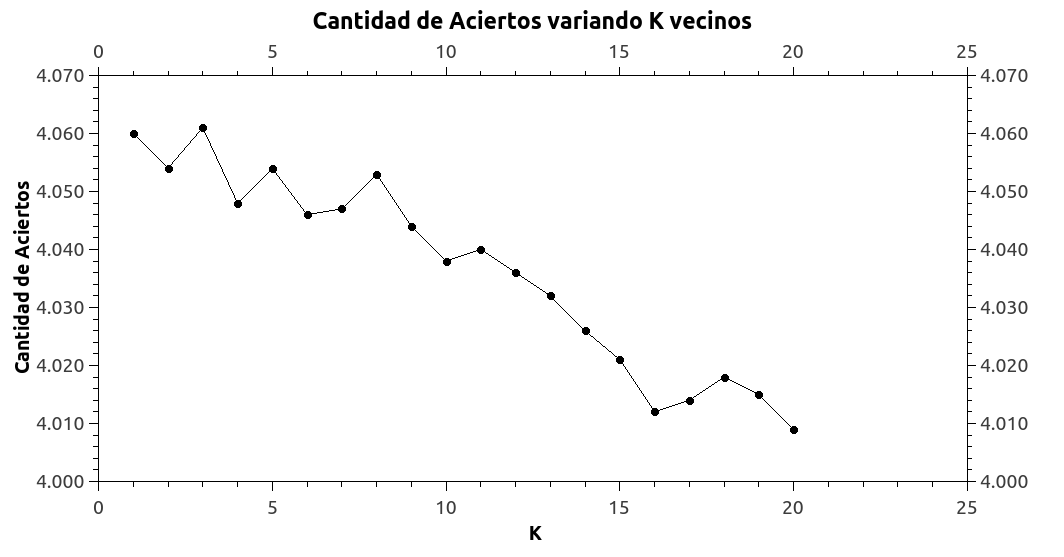
\includegraphics[scale=0.6]{knn.png}
\end{center}

Como se puede observar la iteración que mas aciertos dió es para $K = 3$. Además se puede observar que a medida que se incrementa el valor de $K$ la cantidad de aciertos va disminuyendo levemente, cumpliendo lo mencionado en la introducción teórica. Cuanto mas corta sea la distancia de los vecinos, mas chances hay de tener un acierto.

Luego de los valores obtenidos en base a estas pruebas tomamos las siguientes metricas solicitadas por la catedra.

Prescion: Es una medida de cuantos aciertos relativos tiene un clasificador dentro de una clase particular.

Recall: Es una medida de que tan bueno es un clasificador para, dada una clase particular, identificar correctamente a los pertenecientes a esa clase.


\subsection {Algoritmo de K-NN con Optimización de PCA}
Para el algoritmo de PCA lo que realizamos fue una variacion de los valores de alfa en el algoritmo de pca. para eso $k-fold$ medimos los tiempos de ejecución y los promediamos para poder ver de que manera varía la ejecución de los algoritmos en función de $\alpha$, luego tomamos un promedio de las ejecuciones y obtuvimos lo siguientes resultados:

\begin{center}
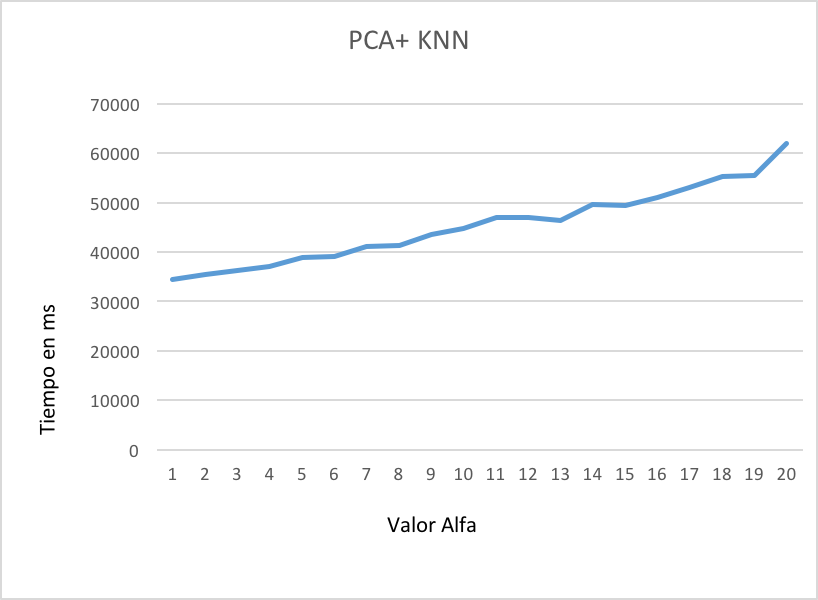
\includegraphics[scale=0.6]{pcaknn.png}
\end{center}

Cabe aclarar que estos tiempos no contemplan todo lo que se considera el ’entrenamiento’ del sistema, es decir, todo el preprocesamiento que resultara en encontrar
los valores principales. La justificacion de esto es que el procedimiento se realizar ́a una vez, para entrenar el sistema y luego, al momento de clasificar las
nuevas imagenes este tiempo podra ser despreciado.Este grafico se puede ver que aumentar el α produce un aumento lineal de los tiempos de ejecucion, 
de lo que se desprende que aumentar la cantidad valores principales no resulta gratuito en t ́erminos de tiempo de ejecuci ́on y tiene cierto costo asociado.


\subsection {Algoritmo de K-NN con Optimización de PSL-DA}
Habiendo fijado k = 3 , corremos el test1.in variando el gamma utilizando los valores 1,2,10 y 50. Aqui el grafico
\begin{figure}[H]
\centering
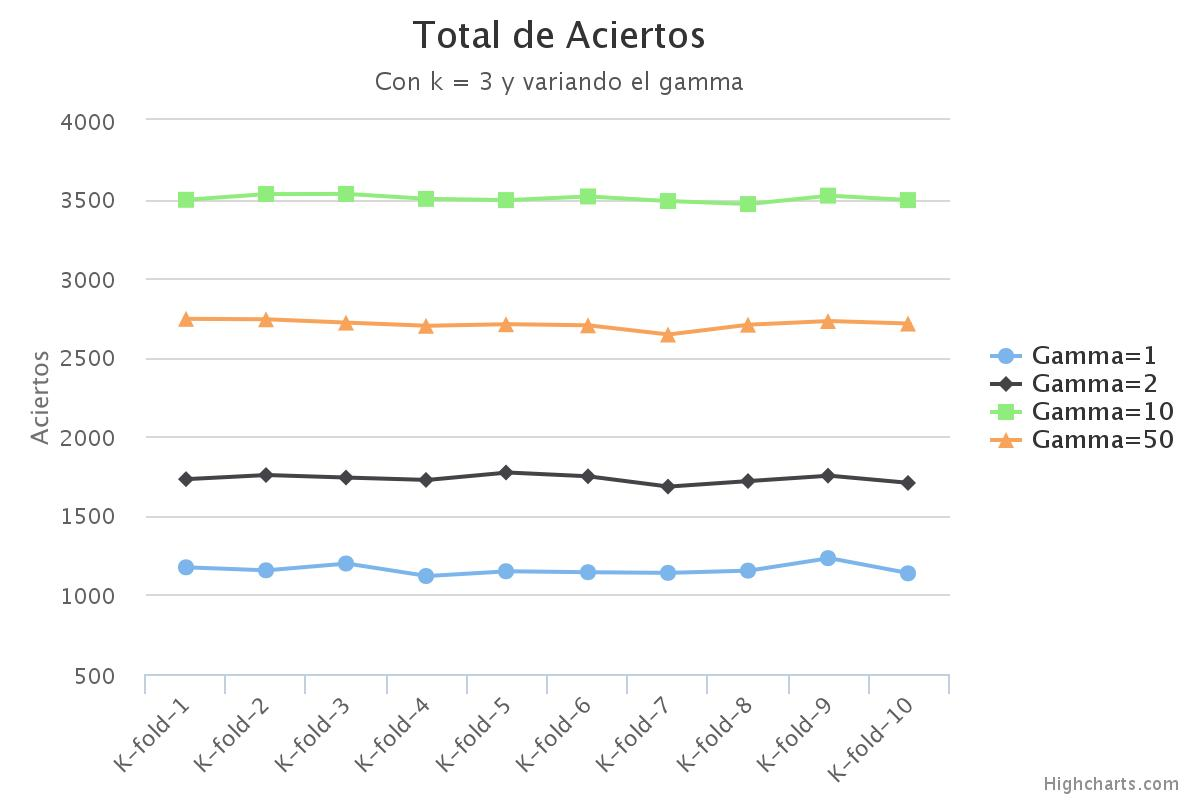
\includegraphics[width=1\textwidth]{chart.jpeg}
\caption{Comparacion de aciertos variando el gamma}
\label{fig:Comparacion de tecnicas}
\end{figure}


Vemos que si aumenta el gamma , mejora la precision pero si gamma aumenta demasiado , en algun momento empeora tu hit rate , suponemos que eso se debe a que si bien tenemos bastante informacion , la cantidad de vecinos no permite aprovecharla . Eso hace suponer que para que tengamos un buen hit rate , debe haber algun tipo de relacion entre el k y el gamma . Eso se va a poner a prueba usando el test2.in

\subsection {Algoritmo de K-NN con Optimización de PSL-DA}

El experimento que nos planteamos es el siguiente. Dejamos fijo el gamma en 13 y hacemos variar el k . Aqui el grafico  
\begin{figure}[H]
\centering
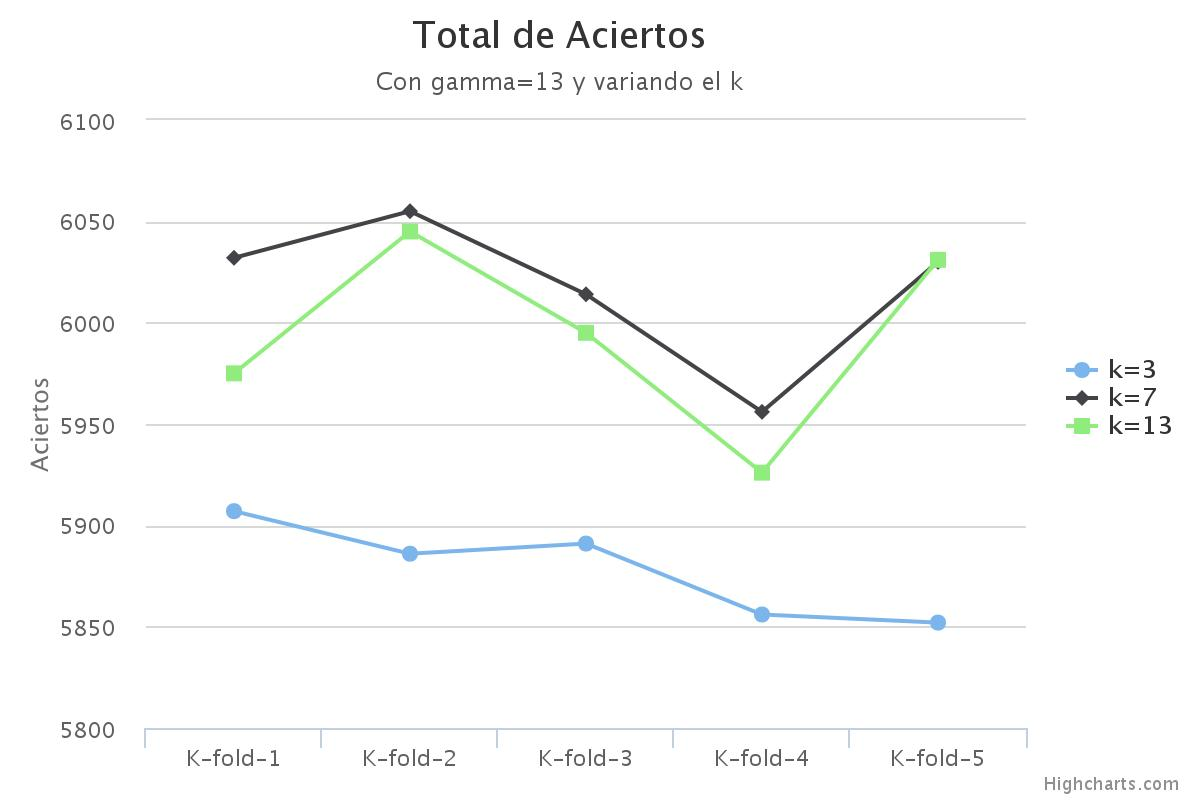
\includegraphics[width=1\textwidth]{chart(2).jpeg}
\caption{Comparacion de aciertos variando el k}
\label{fig:Comparacion de tecnicas}
\end{figure}

De 3 a 7 mejora el hit rate pero es muy poca la mejora en comparacion al aumento de tiempo de computo



